% % !TEX root = ../main.tex
% \chapter{Introduction}
% \label{chapter:Introduction}
% % This document has been created in order to show you some of the capabilities 
% % of \LaTeX.  A great resource for an introduction to \LaTeX\xspace is Tobias
% % Oetiker's ''The Not So Short Introduction to \LaTeXe'' \cite{latex}.  Please
% % page through that document
% % before starting with your thesis.
% % Oh, and let's use the mysterious word \gls{computer} here to give the glossary
% % a reason to appear.
% % A third useful option to reference stuff besides citing or glossarying (?) 
% % is using footnotes. Just like
% % this\footnote{Properly formatted clickable URL: \url{https://www.tum.de/}}
% % one.
% % And: lists! Lists with bullet points are amazing. I mean, just look at this:
% % \begin{itemize}
% % 	\item list
% % 	\item all 
% % 	\item the 
% % 	\item things!
% % \end{itemize}
% % % use enumerate for numbers instead of points: 
% % % https://en.wikibooks.org/wiki/LaTeX/List_Structures#List_structures
% % \par
% % Anyways your introduction goes here.


% % Below a few \LaTeX examples are included for beginners
% % \comment{You can also put comments in the margins for you or your advisor}
% % \begin{figure}[ht]
% %   \centering
% %   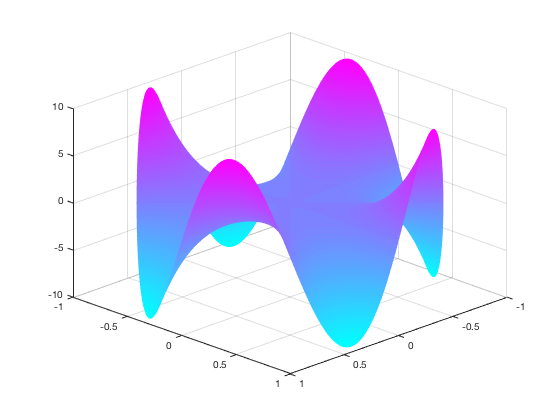
\includegraphics[width=5cm]{images/swing_function_plot.png}
% %   \caption{$u(x)$}%{Numerically solved solution}
% %   \label{fig:swingPlot}
% % \end{figure}


% % Equations can also be labeled
% % \begin{equation}
% % 	\pi = \mathrm{e}^{i\cdot\phi}
% % 	\label{eq:equation1}
% % \end{equation}


% % And later referenced. Even in subfigures.
% % \begin{figure}[!htb]
% %   \centering
% %   \begin{subfigure}[b]{0.3\textwidth}
% %     \centering
% %   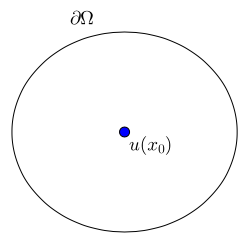
\includegraphics[width=\textwidth]{images/CircCenter}
% %   \caption{Equation~\ref{eq:equation1}}\label{fig:circcenter}
% % \end{subfigure}
% % \hfill
% %   \begin{subfigure}[b]{0.3\textwidth}
% %     \centering
% %   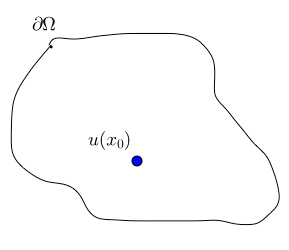
\includegraphics[width=\textwidth]{images/GeneralOffset}
% %   \label{fig:generaloffset}
% %   \caption{Equation~\ref{eq:equation1}}
% % \end{subfigure}
% % \end{figure}
% % \section{Including code}

% % Code can be using the package
% % \href{https://www.sharelatex.com/learn/Code\_Highlighting\_with\_minted}{Minted}.

% % An exaple of which of can be found below (see Source Code~\ref{lst:nice_listing})
% % \begin{listing}
% % 	%the language syntax can be declared here.
% % 	\begin{minted}{python} 
% % 	import numpy as np
	
% % 	def incmatrix(genl1,genl2):
% % 	    m = len(genl1)
% % 	    n = len(genl2)
% % 	    M = None #to become the incidence matrix
% % 	    VT = np.zeros((n*m,1), int)  #dummy variable
	
% % 	    #compute the bitwise xor matrix
% % 	    M1 = bitxormatrix(genl1)
% % 	    M2 = np.triu(bitxormatrix(genl2),1)
	
% % 	    for i in range(m-1):
% % 	        for j in range(i+1, m):
% % 	            [r,c] = np.where(M2 == M1[i,j])
% % 	            for k in range(len(r)):
% % 	                VT[(i)*n + r[k]] = 1;
% % 	                VT[(i)*n + c[k]] = 1;
% % 	                VT[(j)*n + r[k]] = 1;
% % 	                VT[(j)*n + c[k]] = 1;
	
% % 	                if M is None:
% % 	                    M = np.copy(VT)
% % 	                else:
% % 	                    M = np.concatenate((M, VT), 1)
	
% % 	                VT = np.zeros((n*m,1), int)
	
% % 	    return M
% % 	\end{minted}

% %   \caption{My nice listing}
% %   \label{lst:nice_listing}
% % \end{listing}
% Fluid mechanics plays a pivotal role in the progress of various diverse fields, including aerospace and automotive engineering, energy system optimization, environmental modeling, biomedical research, and countless other critical domains that shape our technological and scientific landscape. Partial Differential Equations (PDEs), in particular the Navier-Stokes equations, which provide the mathematical framework for analyzing the behaviour of fluid flow for these complex problems are often intractable, i.e; they do not have exact analytical solutions. Thus, they still remain an open problem in the world of mathematics. Hence, the solutions to the Navier-Stokes equations are approximated using numerical methods such as the Finite Element or the more commonly used Finite Volume Method (FVM) which rely on spatial and temporal discretization of PDEs. With the advent of software and technology, emerged the field of Computational Fluid Dynamics (CFD), leveraging computer algorithms for numerical simulations of fluid flow problems. However, these simulations are computationally intensive and may take from several hours to several weeks for complex flows and/or geometries. Although advances in high-performance computing and parallel processing have been a game-changer for CFD, there still remain several complications with respect to grid dependency, convergence issues, model assumptions and simplification of underlying physics, numerical errors as well as turbulence modelling. \\
% The most problematic use-case is turbulence modelling, which is marked by velocity and pressure fluctuations, a wide range of length and time scales - from large vortices down to small eddies and numerical instabilities. In addition, modelling turbulence near walls presents unique problems on its own which requires specialized treatments and techniques in these near-wall regions. Accurately modelling all the intricate phenomena of the turbulent regime, called the Direct Numerical Simulation (DNS), is possible, but at the cost of a huge amount of computational resources, complexity and simultaion times. Consequently, in many practical scenarios, simplified turbulence models are employed, even though this comes at the expense of accuracy. \\
% Advancements in the dynamic field of CFD over the past had seen substantial efforts channeled into enhancing turbulence models, improving meshing techniques, efficient Reduced Ordered Modelling (ROM) surrogates and reducing computational complexity. While numerous techniques and models exist to address various turbulence-related challenges, there is no universally applicable model that consistently delivers accurate results across all turbulence settings. As a result, the computational bottleneck often remains an unavoidable obstacle. In response to this challenge, in recent times, there has been a growing interest in implementing Machine Learning (ML) algorithms, specifically to enhance the cost-effectiveness of CFD methods. Although training an ML model is often very computationally demanding, a trained model can quickly make predictions on new data, a significant advantage over the commonly used numerical methods. The integration of ML in CFD represents a paradigm shift, enabling simulations to move beyond traditional physics-based models. The synergy between Deep Learning (DL) and CFD offers the potential to uncover novel insights into fluid dynamics, for example, Convolutional Neural Networks (CNNs) can extract relevant features and classify flow regimes whereas Recurrent Neural Networks (RNNs) can predict fluid behaviors based on temporal data for unsteady flows. Incorporating neural networks into fluid dynamics problems not only improves the accuracy and efficiency of simulations, but also opens up new doors for understanding flow behaviours and strategies for flow control and optimization. As neural networks continue to evolve and adapt to the specific challenges of fluid dynamics, they promise to be a pivotal component in the advancement of CFD across various industries and applications. \\
% So far, ML methods have been employed in fluid dynamics research but have not been in engineering practice. Some possible explanations for this might be the scarcity of huge datasets that are open and can be publicly accessed and the poor generalization performance of ML techniques on previously unseen data. This thesis attempts to tackle the generalization problem by implementing a novel approach that combines GNNs with a meta learning principle for accurate and efficient predictions even on unencountered datasets. 
% \section{Literature Review}
% In this section, relevant research and work done with respect to ML in the context of CFD, especially in turbulence modelling is discussed. The evolution of turbulence modeling is a dynamic field with notable milestones and contributions. The pioneering work of Osborne Reynolds in the late 19th century laid the foundation for turbulence research, leading to the eddy viscosity hypothesis and the rise of Reynolds-averaged Navier-Stokes (RANS) modeling in the mid-20th century. The K-epsilon model, introduced in the 1970s, significantly enhanced RANS modeling by striking a balance between accuracy and computational efficiency. Parallel to this development, Large Eddy Simulation (LES) emerged as a complementary approach, aiming to capture large-scale turbulent eddies directly while modeling smaller ones. Advances in computational power enabled the feasibility of LES, particularly for complex geometries and higher Reynolds numbers. Direct Numerical Simulation (DNS), which resolves all turbulent scales, became increasingly attainable due to further advancements in computational resources. Recent research has focused on improving existing models, developing advanced closure schemes, and exploring the use of machine learning techniques. The combination of RANS and LES techniques in hybrid models has also gained traction, offering a promising path towards more efficient and accurate simulations. \\
